%----------------------------------------------------------------------------------------
%    PACKAGES AND THEMES
%----------------------------------------------------------------------------------------
\documentclass[aspectratio=169,xcolor=dvipsnames]{beamer}
\usetheme{CleanEasy}
\usepackage[utf8]{inputenc}
\usepackage{lmodern}
\usepackage[T1]{fontenc}
% \usepackage[brazil]{babel}
\usepackage{fix-cm}
\usepackage{amsmath}
\usepackage{mathtools}
\usepackage{listings}
\usepackage{xcolor}
\usepackage{hyperref}
\usepackage{graphicx} % Allows including images
\usepackage{booktabs} % Allows the use of \toprule, \midrule and \bottomrule in tables
\usepackage{tikz}
\usetikzlibrary{positioning, shapes, arrows, calc, decorations.pathreplacing, arrows.meta, backgrounds, patterns, overlay-beamer-styles}
\usepackage{etoolbox}
\usepackage{animate}
\usepackage{textpos}
\usepackage{transparent}

%----------------------------------------------------------------------------------------
%    LAYOUT CONFIGURATION
%----------------------------------------------------------------------------------------
\pdfstringdefDisableCommands{%
  \def\\{}%
  \def\texttt#1{<#1>}%
}

\newif\ifspecialpage
\specialpagefalse
\addtobeamertemplate{title page}{\specialpagetrue}{\specialpagefalse}

\setbeamertemplate{footline}{
    \leavevmode%
    \hbox{%
        \begin{beamercolorbox}[wd=.2\paperwidth,ht=2.25ex,dp=1ex,left]{title in head/foot}%
            \usebeamerfont{title in head/foot}\hspace*{3ex}\textcolor{fg!30}{Solar Physics + AI}
        \end{beamercolorbox}%
        \begin{beamercolorbox}[wd=.65\paperwidth,ht=1.25ex,dp=1ex,center]{title in head/foot}%
            \usebeamerfont{title in head/foot}\hspace*{-5ex}\textcolor{fg!30}{José P. Marchezi}
        \end{beamercolorbox}%
        \begin{beamercolorbox}[wd=.15\paperwidth,ht=1.25ex,dp=1ex,right]{date in head/foot}%
            \usebeamerfont{date in head/foot}\hspace*{-8ex}\textcolor{fg!30}{\today \hspace*{3ex}
            \insertframenumber{} / \inserttotalframenumber\hspace*{2ex}}
        \end{beamercolorbox}}%
    \vskip0pt\hfill%
}

\AtBeginSection[]
{
  \begin{frame}[plain]
    \begin{tikzpicture}[remember picture,overlay]
      % Fundo limpo
      \fill[MediumBlue!5] (current page.north west) rectangle (current page.south east);
      
      % Título da seção
      \node[
        anchor=west, 
        text width=0.6\paperwidth, 
        align=left, 
        font=\Large\bfseries
      ] at ([xshift=-2cm]current page.center) {
        \insertsectionhead
      };
      
      % Linha horizontal
      \draw[thick, DarkBlue!40] 
        ([xshift=-2cm, yshift=-1cm]current page.center) -- ++(\paperwidth/2,0);
    \end{tikzpicture}
  \end{frame}
}
%----------------------------------------------------------------------------------------
%    TITLE PAGE
%----------------------------------------------------------------------------------------
\title{Automated Solar Filament Segmentation:\\ \large What a Human Baseline Reveals About the Limits}

\author[J. P. Marchezi]{\small{José P. Marchezi\inst{1}}}

\institute[INPE]{\inst{1}National Institute for Space Research, Brasil; \\ \texttt{\scriptsize{\textcolor{fg!50}{jose.marchezi@inpe.br}}}}

\vspace{-2cm}\date{\today}
% Define positions for logos on title page
\titlegraphic{
  \begin{tikzpicture}[remember picture, overlay]
    %EAGE 2025 logo
    % \node[anchor=north west, xshift=-1cm, yshift=-0.3cm] at (current page.north west) {
    %   % 
\includegraphics[height=1cm]{logos/logoGeofisica.jpg}
    % };

    % EAGE logo
    \node[anchor=north east, xshift=-6.2cm, yshift=-0.4cm] at (current page.north east) {
      
\includegraphics[height=0.5cm]{logos/CNPq_v2017_rgb.jpg}
    };
    
    % CEPETRO logo
    \node[anchor=north east, xshift=-0.8cm, yshift=-0.3cm] at (current page.north east) {
      
\includegraphics[height=1.1cm]{logos/inpe_logo.png}
    };


    % % IG logo
    % \node[anchor=north east, xshift=-2.5cm, yshift=-0.3cm] at (current page.north east) {
    %   \includegraphics[height=1.1cm]{logos/LOGO_IG_NAME_D.png}
    % };
    
    %UNICAMP logo
    % \node[anchor=north west, xshift=0cm, yshift=-0.3cm] at (current page.north west) {
    %   
\includegraphics[height=1cm]{logos/baner_esqww.png}
    % };
  \end{tikzpicture}
}


%----------------------------------------------------------------------------------------



\begin{document}

\begin{frame}[plain]
  \titlepage
\end{frame}

\begin{frame}[plain]{Outline}
  \tableofcontents
\end{frame}

%=======================================================================
\section{Why automate filament segmentation}
%=======================================================================

\begin{frame}{Solar filaments}
  \begin{columns}
    \column{0.52\textwidth}
      \begin{itemize}
        \item Cool, dense chromospheric material suspended along magnetic polarity inversion lines.
        \item Seen in absorption against the disk in H$\alpha$: dark, elongated, often with fine side branches (\emph{barbs}).
        \item Their destabilisation is one of the recognised precursors of coronal mass ejections.
        \item Barb orientation tracks the \textbf{sign of magnetic helicity} in the filament channel --- the quantity that governs the field orientation an erupting structure carries into the heliosphere.
      \end{itemize}
    \column{0.48\textwidth}
      \begin{figure}
        \centering
        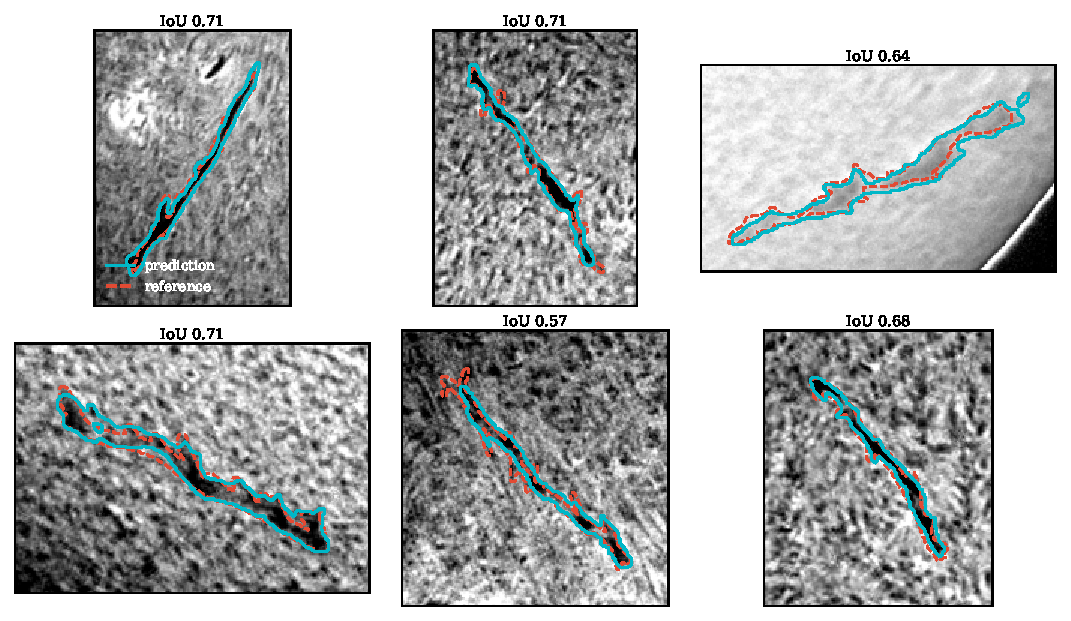
\includegraphics[width=\textwidth]{Figures/filaments/morphology.pdf}
      \end{figure}
      \vspace{-0.5cm}
      \flushright{\tiny{GONG H$\alpha$, native $2048^2$}}
  \end{columns}
\end{frame}

\begin{frame}{The scale problem}
  \begin{columns}
    \column{0.55\textwidth}
      \begin{itemize}
        \item GONG: six stations, full-disk H$\alpha$ roughly once per minute, continuously since 2010.
        \item That is $\sim$3\,900 images \emph{per day}.
        \item MAGFiLO, the reference annotation set, contains \textbf{707} manually annotated images.
        \item Ratio: humans have annotated about \textbf{four hours} of what the network has observed in fifteen years.
      \end{itemize}
      \vspace{0.3cm}
      \small{Automation is not a convenience here. It is the only way a filament catalogue can exist at the cadence the observations are taken.}
    \column{0.45\textwidth}
      \begin{block}{What a catalogue would enable}
        \small
        Filament statistics across the solar cycle; eruption precursor studies at scale; and operational monitoring, where what matters is noticing a large filament \emph{before} it erupts.
      \end{block}
  \end{columns}
\end{frame}

\begin{frame}{Semantic is not enough: the task is \emph{instance} segmentation}
  \begin{columns}
    \column{0.5\textwidth}
      \textbf{Semantic segmentation} answers: \emph{is this pixel filament material?}
      \begin{itemize}\small
        \item Gives a binary map of the disk.
        \item Cannot say how many filaments there are, or where one ends and the next begins.
      \end{itemize}
      \vspace{0.3cm}
      \textbf{Instance segmentation} answers: \emph{which filament is this pixel part of?}
      \begin{itemize}\small
        \item Required for any per-filament quantity: length, area, latitude, chirality, lifetime.
        \item A catalogue needs objects, not a mask.
      \end{itemize}
    \column{0.5\textwidth}
      \begin{alertblock}{The hard part}
        \small A single physical filament frequently appears as several disconnected dark patches. Deciding they are \emph{one} object is a judgement call --- and it is where naive methods fail.
      \end{alertblock}
  \end{columns}
\end{frame}

%=======================================================================
\section{The data, and how performance is measured}
%=======================================================================

\begin{frame}{MAGFiLO}
  \begin{columns}
    \column{0.55\textwidth}
      \begin{itemize}
        \item 1\,154 annotation \emph{records} over \textbf{707 photographs}: up to three experts annotate the same image independently.
        \item 42\,\% of images carry more than one annotator.
        \item Each annotation: polygon, bounding box, \textbf{spine polyline}, and a \textbf{chirality} label.
        \item Splits must be made at the level of the photograph --- splitting on record identifiers leaks the same pixels into both sides.
      \end{itemize}
    \column{0.45\textwidth}
      \begin{figure}
        \centering
        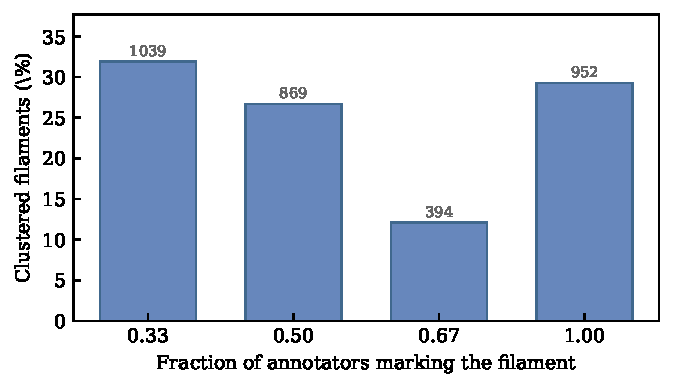
\includegraphics[width=\textwidth]{Figures/filaments/annotator_agreement.pdf}
      \end{figure}
      \vspace{-0.4cm}
      \flushright{\tiny{3\,254 clustered filaments, 296 multi-annotator images}}
  \end{columns}
  \vspace{0.2cm}
  \small{\textbf{Experts disagree about \emph{whether} a darkening is a filament}, not only about its boundary: only 29\,\% of distinct filaments are marked by all available annotators.}
\end{frame}

\begin{frame}{Panoptic Quality}
  \[
    \mathrm{PQ}=\underbrace{\frac{\sum_{\mathrm{TP}}\mathrm{IoU}}{|\mathrm{TP}|}}_{\displaystyle \mathrm{SQ}}\;\times\;
    \underbrace{\frac{|\mathrm{TP}|}{|\mathrm{TP}|+\tfrac12|\mathrm{FP}|+\tfrac12|\mathrm{FN}|}}_{\displaystyle \mathrm{RQ}}
  \]
  \vspace{0.2cm}
  \begin{columns}
    \column{0.5\textwidth}
      \begin{itemize}\small
        \item Instances match at $\mathrm{IoU}>0.5$; counts pooled globally, not averaged per image.
        \item \textbf{SQ} --- how well we delineate what we found.
        \item \textbf{RQ} --- how well we find what is there.
      \end{itemize}
    \column{0.5\textwidth}
      \begin{block}{Why the factorisation matters}
        \small The two move independently. A single PQ number hides which one is binding --- and in this work they turn out to have completely different ceilings.
      \end{block}
  \end{columns}
\end{frame}

\begin{frame}{An aside that cost us more than any model change}
  \begin{columns}
    \column{0.45\textwidth}
      \small
      Ground-truth polygons must be rasterised to masks. Two standard ways disagree:
      \begin{itemize}\small
        \item \texttt{cv2.fillPoly} vs \texttt{pycocotools}
        \item mean IoU between them: \textbf{0.876} over all 8\,199 annotations
        \item OpenCV masks systematically larger
        \item boundary effect $\Rightarrow$ worst on thin objects: \textbf{0.850} below median area vs \textbf{0.901} above
      \end{itemize}
      \vspace{0.2cm}
      Correcting the convention moved our score more than any architectural change we tried.
    \column{0.55\textwidth}
      \begin{figure}
        \centering
        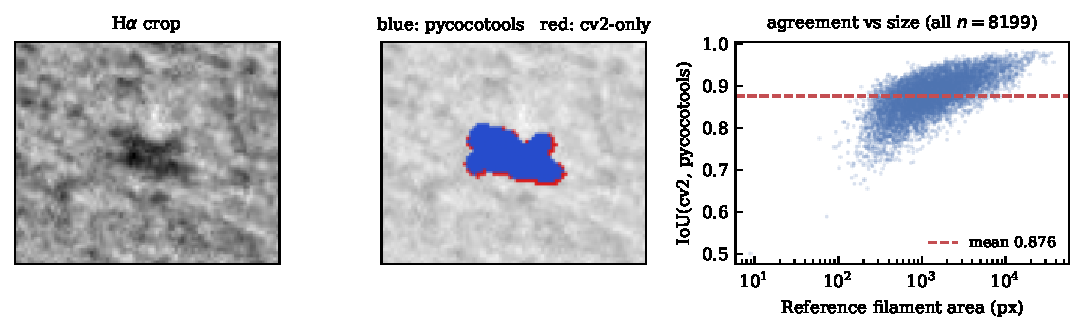
\includegraphics[width=\textwidth]{Figures/filaments/rasterization.pdf}
      \end{figure}
  \end{columns}
\end{frame}

%=======================================================================
\section{What we built}
%=======================================================================

\begin{frame}{MaskStitch: detect -- crop -- refine}
  \begin{figure}
    \centering
    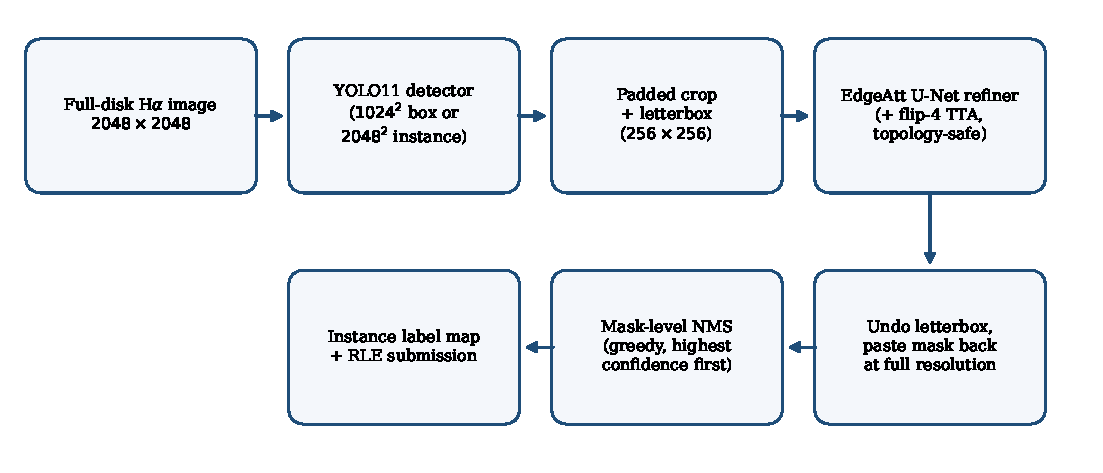
\includegraphics[width=0.92\textwidth]{Figures/filaments/pipeline.pdf}
  \end{figure}
  \vspace{-0.2cm}
  \begin{columns}
    \column{0.5\textwidth}
      \begin{itemize}\small
        \item \textbf{Detect}: YOLO11 instance segmentation at native $2048^2$ proposes each filament.
        \item \textbf{Crop}: padded, letterbox-resized to $256^2$ --- aspect ratio preserved, since a square crop of a thin diagonal object is mostly empty margin.
      \end{itemize}
    \column{0.5\textwidth}
      \begin{itemize}\small
        \item \textbf{Refine}: compact U-Net with an edge-guided attention bottleneck; prediction averaged over four flips when that preserves mask topology.
        \item \textbf{Stitch}: greedy suppression computed on the \emph{masks}.
      \end{itemize}
  \end{columns}
\end{frame}

\begin{frame}{Why suppression must happen in mask space}
  \begin{columns}
    \column{0.5\textwidth}
      \begin{itemize}
        \item Standard practice resolves duplicate detections by bounding-box overlap.
        \item For a long, thin, \emph{diagonal} object, the box is mostly background: two detections of the same filament can have low box IoU, and two different filaments can have high box IoU.
        \item We suppress on the masks instead: a candidate already mostly claimed by a higher-confidence instance is rejected, not admitted as a fragment.
      \end{itemize}
    \column{0.5\textwidth}
      \begin{exampleblock}{Consequence}
        \small
        Fragmentation (one filament split across predictions): \textbf{0.6\,\%}\\[2pt]
        Over-merging (one prediction absorbing several filaments): \textbf{2.2\,\%}\\[6pt]
        Structural continuity is the difficulty the challenge organisers list third --- and it is where this design is strongest.
      \end{exampleblock}
  \end{columns}
\end{frame}

%=======================================================================
\section{Results}
%=======================================================================

\begin{frame}{Overall performance}
  \begin{columns}
    \column{0.52\textwidth}
      \small
      \begin{tabular}{lr}
        \toprule
        Panoptic Quality & 0.4571 \\
        \quad SQ (mean IoU of matches) & 0.674 \\
        \quad RQ & 0.678 \\
        \midrule
        Matched pairs & 222 \\
        \quad mean Dice & 0.802 \\
        \midrule
        Reference missed & 22.1\,\% \\
        Predictions spurious & 18.4\,\% \\
        Fragmented & 0.6\,\% \\
        Over-merged & 2.2\,\% \\
        \midrule
        Median area, pred / ref & 1251 / 1251\,px \\
        \bottomrule
      \end{tabular}
    \column{0.48\textwidth}
      \begin{figure}
        \centering
        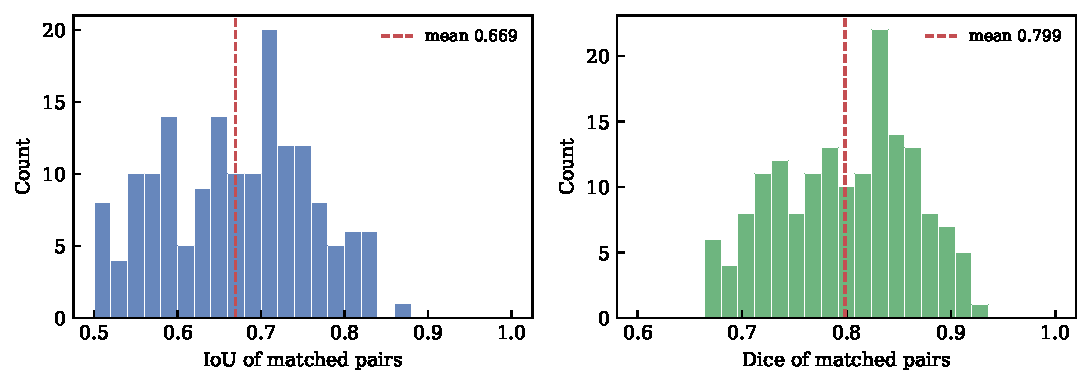
\includegraphics[width=\textwidth]{Figures/filaments/distributions.pdf}
      \end{figure}
      \vspace{-0.3cm}
      \begin{figure}
        \centering
        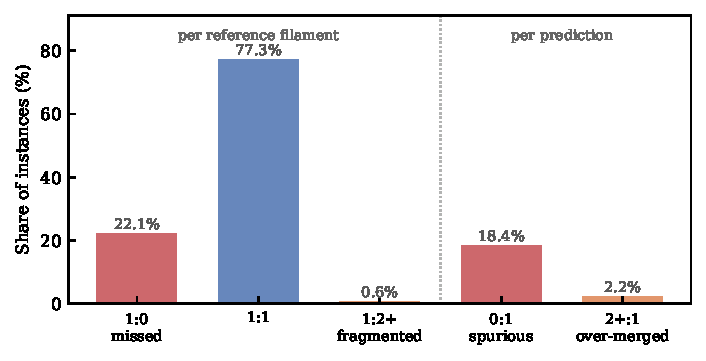
\includegraphics[width=\textwidth]{Figures/filaments/m2n_relations.pdf}
      \end{figure}
  \end{columns}
\end{frame}

\begin{frame}{What the predictions look like}
  \begin{figure}
    \centering
    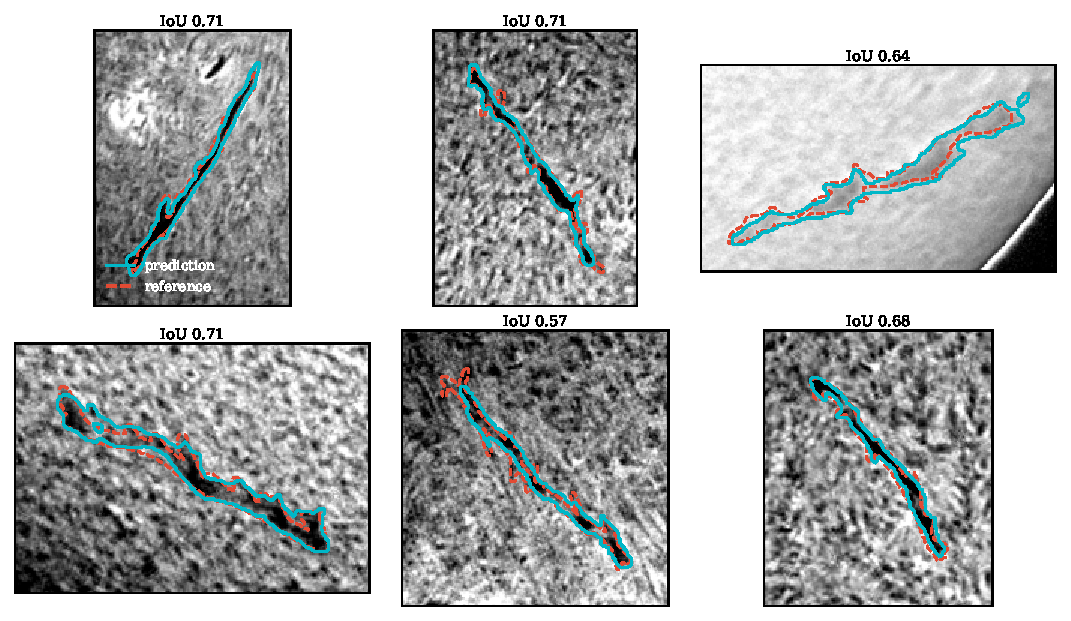
\includegraphics[width=0.85\textwidth]{Figures/filaments/morphology.pdf}
  \end{figure}
  \vspace{-0.2cm}
  \small{Contours follow the spine and its branchings rather than enclosing a convex envelope. The third panel is a near-limb case. The predicted outline sits marginally \emph{outside} the reference --- under a matching rule with an IoU cut, over-covering slightly is safer than under-covering.}
\end{frame}

%=======================================================================
\section{How good is good? A human baseline}
%=======================================================================

\begin{frame}{The question nobody in this literature asks}
  \begin{columns}
    \column{0.55\textwidth}
      Every published filament segmenter is scored against \emph{one} reference annotation, and reports a number.
      \vspace{0.3cm}
      \begin{alertblock}{But}
        If two experts annotating the same image disagree, then part of every reported error is not error at all --- and nobody has measured how large that part is.
      \end{alertblock}
      \vspace{0.3cm}
      MAGFiLO's multi-annotator structure lets us measure it \textbf{under the same metric used to score machines}.
    \column{0.45\textwidth}
      \begin{block}{Two protocols}
        \small
        \textbf{Boundary agreement}: for every pair of annotators and every filament both identified, record the IoU between their delineations.\\[4pt]
        \textbf{Annotator as predictor}: the task is to predict one held-out annotator's labels. The competitor is another annotator.
      \end{block}
  \end{columns}
\end{frame}

\begin{frame}{The ceiling is the label, not the model}
  \begin{columns}
    \column{0.5\textwidth}
      \begin{itemize}
        \item Two experts agree on a commonly identified filament at a mean IoU of \textbf{0.631} \\ {\small(95\,\% CI $[0.625,\,0.636]$, 4\,290 matched pairs)}
        \item Our model's SQ against held-out annotations: \textbf{0.665}
      \end{itemize}
      \vspace{0.3cm}
      \begin{exampleblock}{}
        \small Automated masks already agree with the reference \textbf{at least as closely as a second expert does}. There is no headroom left in boundary placement: a model scoring materially higher would be reproducing one annotator's idiosyncrasy, not becoming more accurate.
      \end{exampleblock}
    \column{0.5\textwidth}
      \begin{block}{Asked symmetrically}
        Predicting one held-out annotator's labels:
        \vspace{0.2cm}
        \begin{tabular}{lc}
          \toprule
          & PQ \\
          \midrule
          Another human expert & 0.341 \\
          Our model & \textbf{0.430} \\
          \bottomrule
        \end{tabular}
        \vspace{0.2cm}
        \small Read carefully: the model is trained on pooled annotations, so it predicts the \emph{consensus} --- which lies closer to any individual than another individual does. This is a statement about consensus, not about perception.
      \end{block}
  \end{columns}
\end{frame}

\begin{frame}{But SQ is not RQ}
  \begin{columns}
    \column{0.5\textwidth}
      \textbf{Segmentation quality} has reached the human level. \\
      \textbf{Recognition quality} has not.
      \vspace{0.3cm}
      \begin{itemize}\small
        \item Recall tracks expert consensus: \textbf{0.31} for filaments one expert of three marked, \textbf{0.86} for those all experts confirmed.
        \item What we miss is systematically \textbf{small and faint} --- and those are the filaments the annotators themselves disagree about.
        \item Of 119 unmatched references, \textbf{56\,\% receive no overlapping proposal at all}. Only 19\,\% sit just below the matching cut.
      \end{itemize}
    \column{0.5\textwidth}
      \begin{figure}
        \centering
        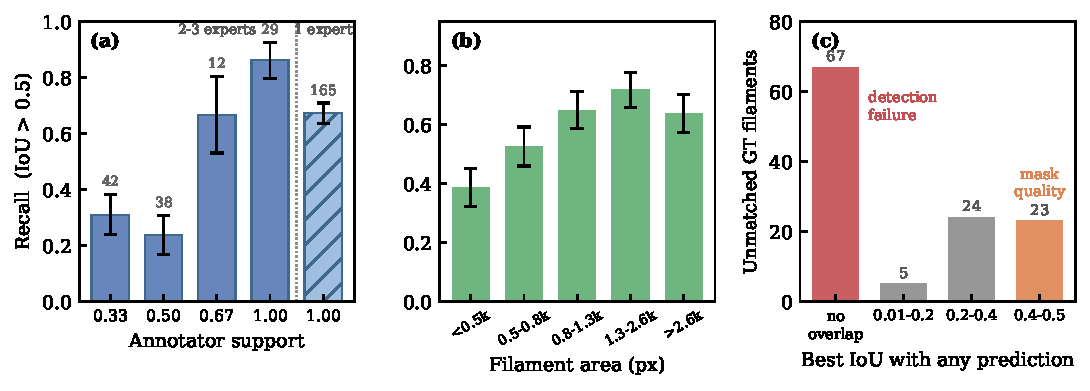
\includegraphics[width=\textwidth]{Figures/filaments/failures.pdf}
      \end{figure}
      \vspace{-0.2cm}
      \flushright{\tiny{Held-out split, 286 consensus-clustered filaments}}
  \end{columns}
\end{frame}

%=======================================================================
\section{Ten things that did not work}
%=======================================================================

\begin{frame}{A controlled search}
  \begin{columns}
    \column{0.42\textwidth}
      \small
      Eighteen configurations, six independent design axes, one held-out partition, one metric implementation, each with its own threshold sweep.
      \vspace{0.25cm}
      \begin{itemize}\small
        \item Detector architecture: 9M @1024 vs 27.6M @2048 $\rightarrow$ \textbf{0.002}
        \item Refiner capacity: $+$75\,\% parameters $\rightarrow$ $+0.009$ crop Dice, \textbf{$+0.000$ PQ}
        \item Annotator-merge target, learned re-scorer, extra proposal source, crop context $\rightarrow$ all null
      \end{itemize}
    \column{0.58\textwidth}
      \begin{figure}
        \centering
        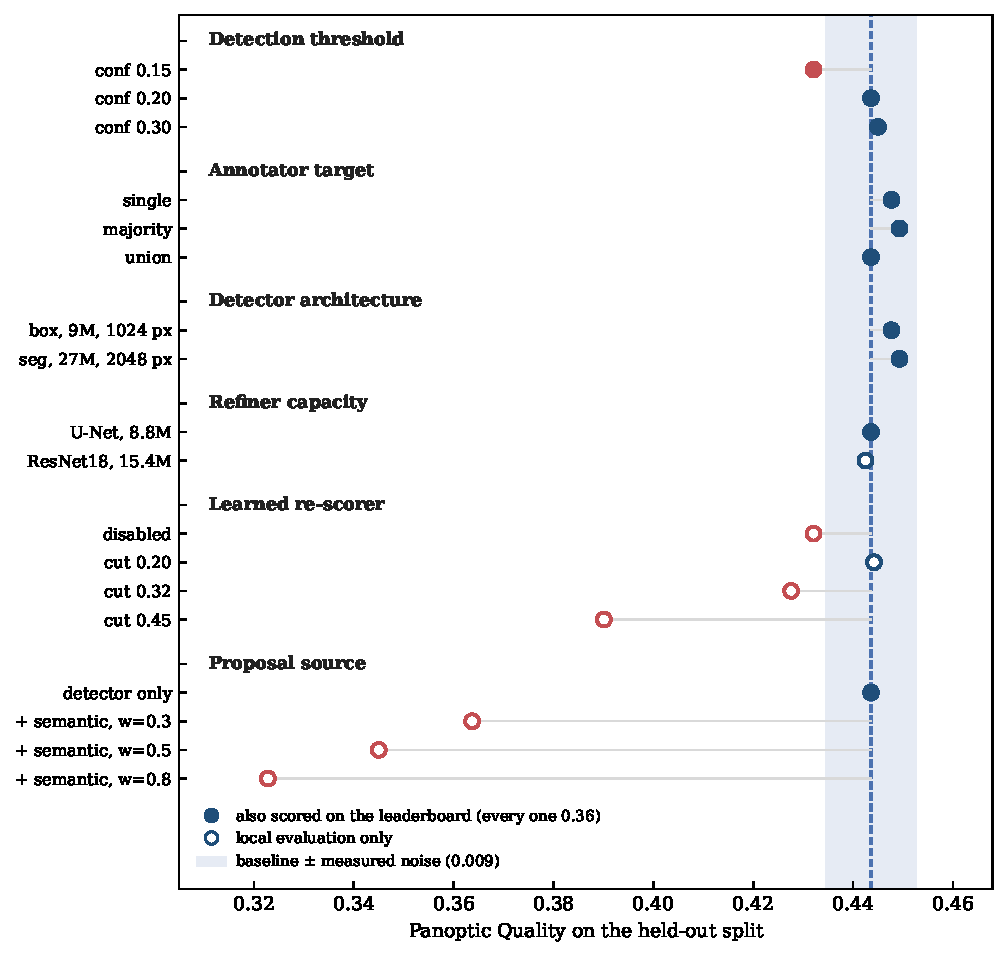
\includegraphics[width=\textwidth]{Figures/filaments/interventions.pdf}
      \end{figure}
  \end{columns}
\end{frame}

\begin{frame}{Can unlabelled data substitute for labels?}
  \begin{columns}
    \column{0.45\textwidth}
      \small
      2\,500 further GONG H$\alpha$ images, 2011--2022, six stations, verified disjoint from every annotated image.
      \vspace{0.2cm}
      Pseudo-labels by three selection rules, detector retrained from scratch each time, validation kept real.
      \vspace{0.3cm}
      \begin{alertblock}{Label density governs the outcome}
        \small Below $\sim$75\,\% of the true density, every unlabelled filament is trained as \emph{background} and the detector learns to stay silent: miss rate 21\,\%\,$\rightarrow$\,37\,\%, false positives halved.
      \end{alertblock}
    \column{0.55\textwidth}
      \begin{figure}
        \centering
        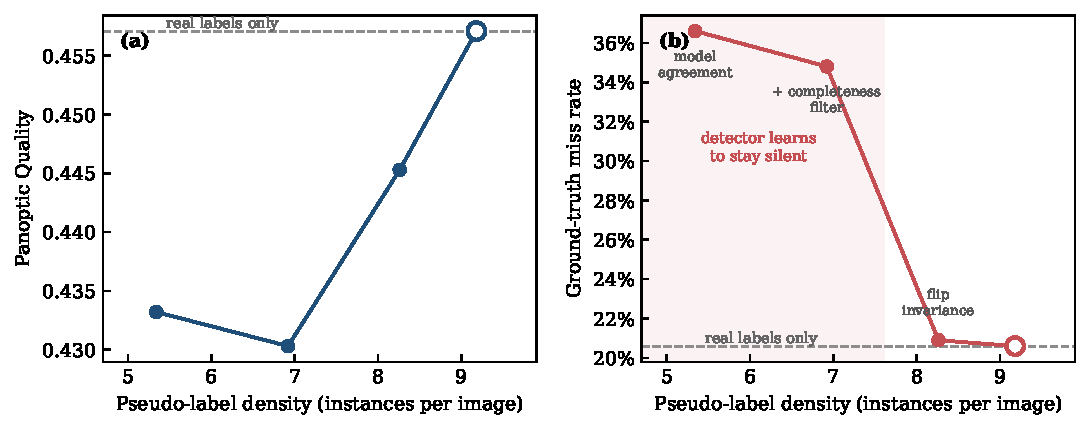
\includegraphics[width=\textwidth]{Figures/filaments/semisup.pdf}
      \end{figure}
      \vspace{-0.3cm}
      \small{At 90\,\% density the collapse vanishes --- and there is still no gain. Model-generated targets carry no information the model lacks.}
  \end{columns}
\end{frame}

\begin{frame}{What the nulls mean}
  \begin{columns}
    \column{0.55\textwidth}
      \begin{itemize}
        \item Ten axes varied, spanning a factor of three in model capacity and four in input resolution. None cleared the measured noise floor of $\pm0.009$.
        \item The only change that did: retuning two \emph{inference} thresholds \textbf{jointly} rather than one at a time ($+0.014$).
        \item Two constants we had treated as task properties --- the mask threshold and the crop context --- are properties of the \emph{trained weights}. A mismatch of 0.25 in crop context costs 0.08 PQ.
      \end{itemize}
    \column{0.45\textwidth}
      \begin{exampleblock}{The reading}
        \small
        We can \emph{localise} about 90\,\% of filaments --- the union of two independent proposal sources proves it.
        \vspace{0.2cm}
        What we cannot do is \textbf{decide} which proposals are real. Every route that raised recall lost precision faster.
      \end{exampleblock}
  \end{columns}
\end{frame}

%=======================================================================
\section{A physical result hiding in the labels}
%=======================================================================

\begin{frame}{The field every pipeline throws away}
  \begin{columns}
    \column{0.55\textwidth}
      \begin{itemize}
        \item MAGFiLO's category field is not a nuisance label: it records filament \textbf{chirality}, assigned from barb bearing relative to the spine.
        \item 30.9\,\% sinistral, 31.6\,\% dextral, 37.5\,\% undetermined.
        \item Chirality is a proxy for the \textbf{sign of magnetic helicity} in the filament channel.
        \item Every segmentation pipeline we are aware of --- including ours --- collapses this to a single class and discards it.
      \end{itemize}
    \column{0.45\textwidth}
      \begin{block}{Does the label carry physics?}
        \small
        Martin (1998) and Pevtsov et al.\ (2003): dextral filaments dominate the northern hemisphere, sinistral the southern, largely independently of the solar cycle.
        \vspace{0.2cm}
        If the annotations reproduce that, they encode a real magnetic property --- not annotator convention.
      \end{block}
  \end{columns}
\end{frame}

\begin{frame}{The hemispheric rule, recovered from the annotations}
  \begin{figure}
    \centering
    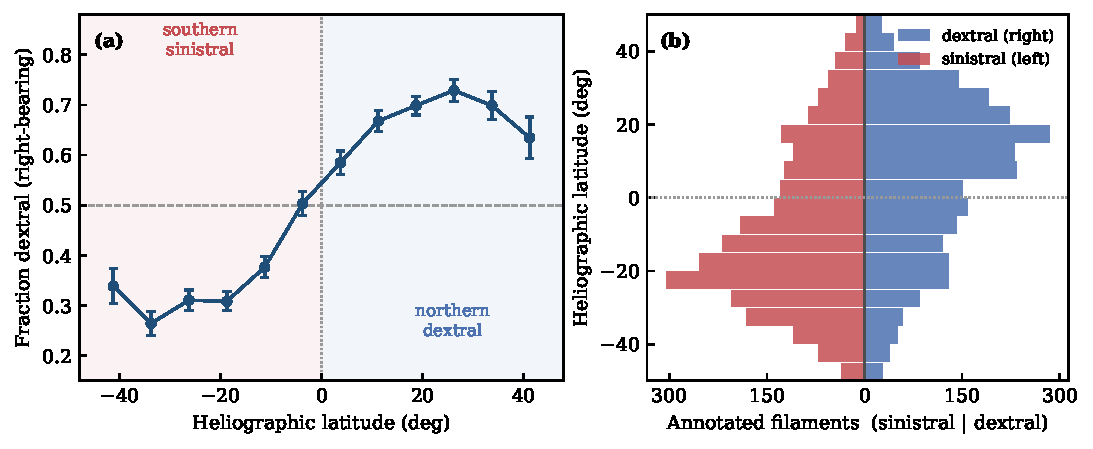
\includegraphics[width=0.88\textwidth]{Figures/filaments/chirality.pdf}
  \end{figure}
  \vspace{-0.25cm}
  \begin{columns}
    \column{0.55\textwidth}
      \small
      5\,125 filaments, 2011--2022. GONG frames are not rotated to solar north, so the position angle $P$ and the $B_0$ projection must be removed first (Meeus 1998, validated against the ephemeris).
    \column{0.45\textwidth}
      \small
      \textbf{67.0\,\%} of northern filaments dextral; \textbf{64.3\,\%} of southern sinistral; $\chi^2=503$ on 1 d.o.f.\\
      The curve crosses one half \textbf{at the equator}.
  \end{columns}
\end{frame}

\begin{frame}{Why this matters operationally}
  \begin{columns}
    \column{0.55\textwidth}
      \begin{itemize}
        \item The sign of magnetic helicity determines the field orientation an erupting filament carries into the heliosphere --- and therefore whether the resulting magnetic cloud is geoeffective.
        \item A segmenter that returns chirality alongside the outline is worth more to a forecaster than one returning position alone.
        \item The supervision is \textbf{already in the dataset}, at no additional annotation cost.
      \end{itemize}
    \column{0.45\textwidth}
      \begin{exampleblock}{And the undetermined class is data, too}
        \small
        The 37.5\,\% the experts declined to classify are not noise to be imputed. They are a \textbf{measurement of where barb geometry is unreadable in H$\alpha$} --- which is itself worth knowing.
      \end{exampleblock}
  \end{columns}
\end{frame}

%=======================================================================
\section{Implications and outlook}
%=======================================================================

\begin{frame}{For operational monitoring}
  \begin{columns}
    \column{0.52\textwidth}
      \begin{itemize}
        \item \textbf{Throughput is not the obstacle}: 7.6 full-disk images per second with test-time augmentation, against a GONG cadence of $\sim$0.1 per second. Seventy-six times the headroom.
        \item \textbf{But the metric is not the mission.} PQ penalises a missed filament and a spurious one equally. A forecaster does not: a missed erupting filament costs a warning; a false alarm costs a glance.
        \item Recall by size: \textbf{38.6\,\%} for the smallest quintile, \textbf{63.8\,\%} for the largest. We miss more than a third of the large filaments --- the ones that erupt.
      \end{itemize}
    \column{0.48\textwidth}
      \begin{alertblock}{Honest caveat}
        \small
        Everything here is validated on GONG H$\alpha$ from one period, train and test drawn from the same distribution. Drift across the solar cycle, instrument changes, or filter degradation at one station are real failure modes none of our numbers cover.
      \end{alertblock}
  \end{columns}
\end{frame}

\begin{frame}{Three lessons that generalise}
  \begin{enumerate}
    \item \textbf{Report the human baseline.} On multi-annotator data it costs nothing beyond the annotations already collected, and it contextualises every other number. Without it we would have spent months chasing SQ that was already at the ceiling.
    \vspace{0.25cm}
    \item \textbf{State the evaluation conventions.} The polygon rasterisation convention is worth several points of IoU on thin structures and cannot be inferred from a reported metric. Inference constants are properties of the weights, not of the task.
    \vspace{0.25cm}
    \item \textbf{A benchmark score is not a measurement} until you know what produced it. Of the public entries above ours on the leaderboard, the ones we could inspect emit a hard-coded payload rather than running the model they display.
  \end{enumerate}
\end{frame}

\begin{frame}{Conclusions}
  \begin{columns}
    \column{0.52\textwidth}
      \begin{itemize}
        \item A detect--crop--refine pipeline reaching $\mathrm{PQ}=0.457$ on held-out data, with fragmentation and over-merging both under 3\,\%.
        \item \textbf{Mask quality is at the level of expert agreement}: SQ 0.665 against 0.631 between two experts.
        \item \textbf{Recognition is not}, and the gap is not addressable by capacity: ten design axes, all null.
        \item The annotations reproduce the hemispheric chirality rule --- physics that every pipeline currently discards.
      \end{itemize}
    \column{0.48\textwidth}
      \begin{block}{What we would do next}
        \small
        Supervision from the spine polylines MAGFiLO already distributes, which no pipeline consumes; and a chirality-aware segmenter, which would return the helicity sign at no extra annotation cost.
      \end{block}
      \vspace{0.3cm}
      \small
      \textbf{Code, weights and a notebook that regenerates the submitted predictions byte for byte:}\\
      {\scriptsize\texttt{github.com/ClimaEspacial/solar\_filaments\_detection}}
  \end{columns}
\end{frame}

\begin{frame}[plain]
  \begin{center}
    {\Huge Thank you}\\[0.6cm]
    {\large Questions?}\\[1cm]
    {\small José P. Marchezi --- \texttt{jose.marchezi@inpe.br}}
  \end{center}
\end{frame}

\end{document}
